\section{Galactic kinematics}\label{sect:galactickinematics}

%Firstly an introduction to galaxies is given, and afterwards galactic formation and evolution models are considered. This is followed with a discussion on how the theories form predictions that call for observations to constrain the theories.
%
%\subsection{Galaxies}
%
%Galaxies have been called the building blocks of the Universe and are in general seen as the home of stars. Knowing a few basic facts about galaxies, and in particular our own galaxy, the Milky Way, is beneficial to getting an idea of the overarching astronomical context of the work discussed in this thesis.
%
%A galaxy typically has a radius of the order of several kpc and a mass, not including dark matter, between $10^{7}$\,M$_\odot$ and $10^{12}$\,M$_\odot$ and is self gravitating. The Milky Way galaxy is estimated to have a radius of about $25\pm10$\,kpc with the Sun located about 8\,kpc from the centre and has a mass of stars and other baryonic material of about $6 \cdot 10^{10}$\,M$_\odot$. Extending the radius out to about 200\,kpc and including the dark matter halo the mass of the Milky Way reaches upwards to $10^{12}$\,M$_\odot$ \citep{blandhawthorn:16}.
%
%Galaxies come in various forms and shapes and the two dominant classifications are spherical and spiral galaxies, often called respectively early type and late type galaxies. The classifications can further be subdivided, for example a spiral galaxy can have a bar or not, and there can be several disk components. The Milky Way is considered to be be a barred spiral galaxy with a bulge and both a thin and thick disk surrounded by a halo, as illustrated in Figure~\ref{fig:milkywaysketch}.
%\begin{figure}[t]
%    \centering
%    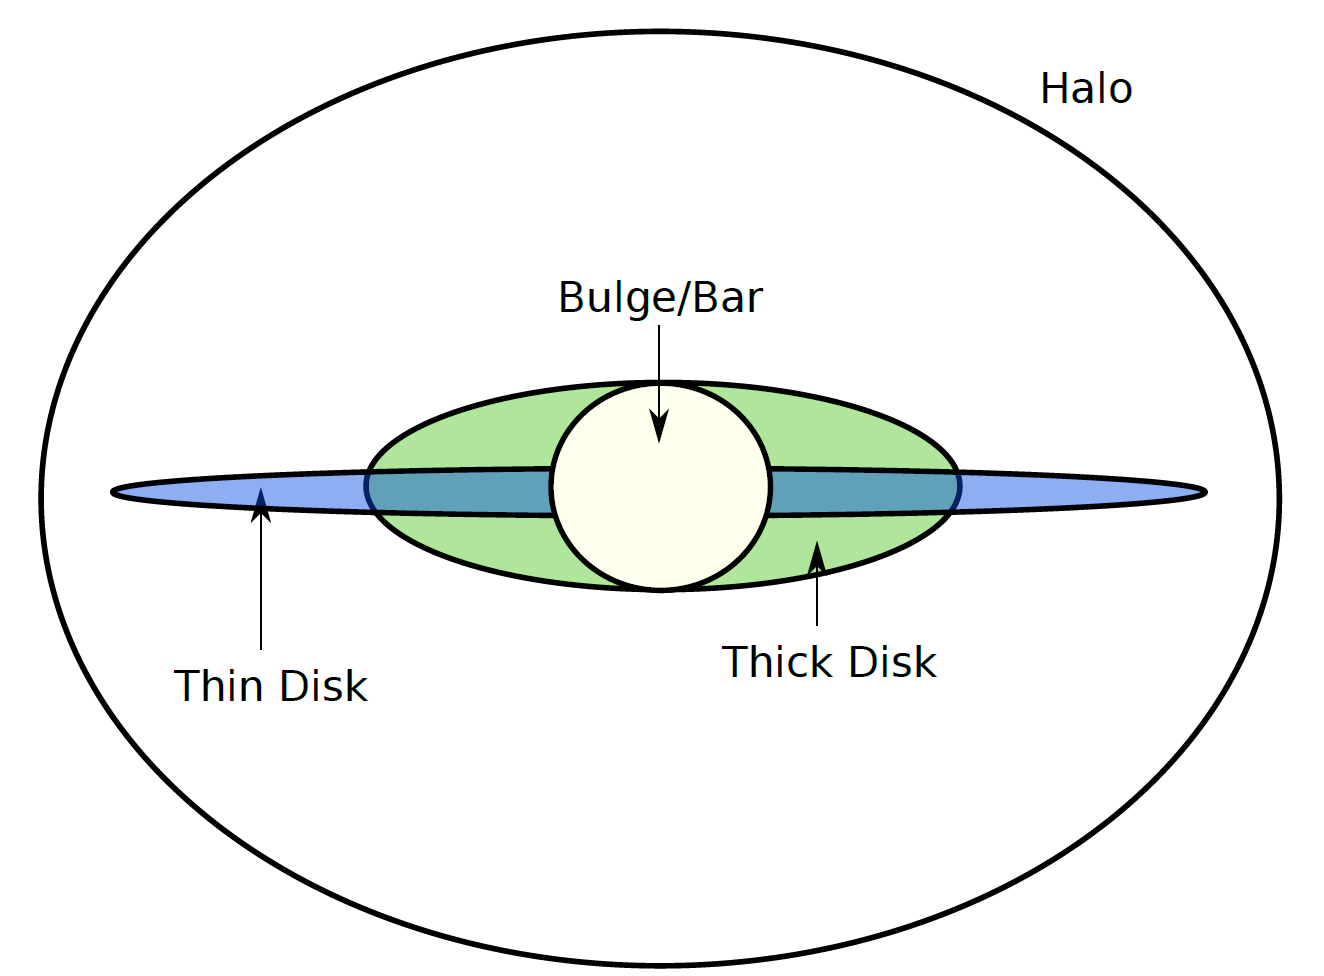
\includegraphics[width=0.8\textwidth]{images/milkywaysketch.png}
%    \caption{A schematic illustration of the stellar components of the Milky Way. The thick disk is illustrated in green, the thin disk in blue and the bulge/bar in beige. The stellar halo surrounding it all is in white. Adapted from \citet{ivalubarlachchristensen:master} with permission.} % Fig. 1.1
%    \label{fig:milkywaysketch}
%\end{figure}
%The bulge is thought to have a mass of about $1.8 \cdot 10^{10}$\,M$_\odot$, the thin disk about $3.5 \cdot 10^{10}$\,M$_\odot$, the thick disk about $6 \cdot 10^9$\,M$_\odot$ and the stellar halo about $4$-$7 \cdot 10^8$\,M$_\odot$ \citep{blandhawthorn:16}.
%
%Almost all galaxies we observe have a bright stellar nucleus, a so-called nuclear star cluster, at their centre \citep{neumayer:20}. The Milky Way is no exception, and has a nuclear star cluster with a radius of about 5\,pc having a mass of about $2.5 \cdot 10^7$\,M$_\odot$. Surrounding the nuclear star cluster is a nuclear stellar disk that extends out towards $150$-$200$\,pc radius and has a mass of about $1.5 \cdot 10^9$\,M$_\odot$ \citep{blandhawthorn:16}. Note, that the distances are now of the orders of pc instead of kpc, which serves to illustrate that these regions have a very high density of stars. At the centre of the nuclear star cluster in the Milky Way lies a supermassive black hole with the mass of about $4.2 \cdot 10^6$\,M$_\odot$ \citep{blandhawthorn:16}. Supermassive black holes have been detected in many galaxies, but are not as ubiquitous as nuclear star clusters \citep{neumayer:20}.
%
%Nuclear star clusters have been found to have empirical relations with their host galaxy, suggesting that nuclear star clusters may have coevolved with their host. Studying nuclear star clusters thus potentially becomes key in understanding the galaxies they are located in, which is particularly interesting as nuclear star clusters are very dense star environments making them bright targets that can be observed from much further away compared to other parts of their host galaxy. One particularly interesting relationship is that between the mass of the nuclear star cluster and the mass of its host. The mass relationship is shown in Figure~\ref{fig:nscrelation}.
%
%\begin{figure}[t]
%    \centering
%    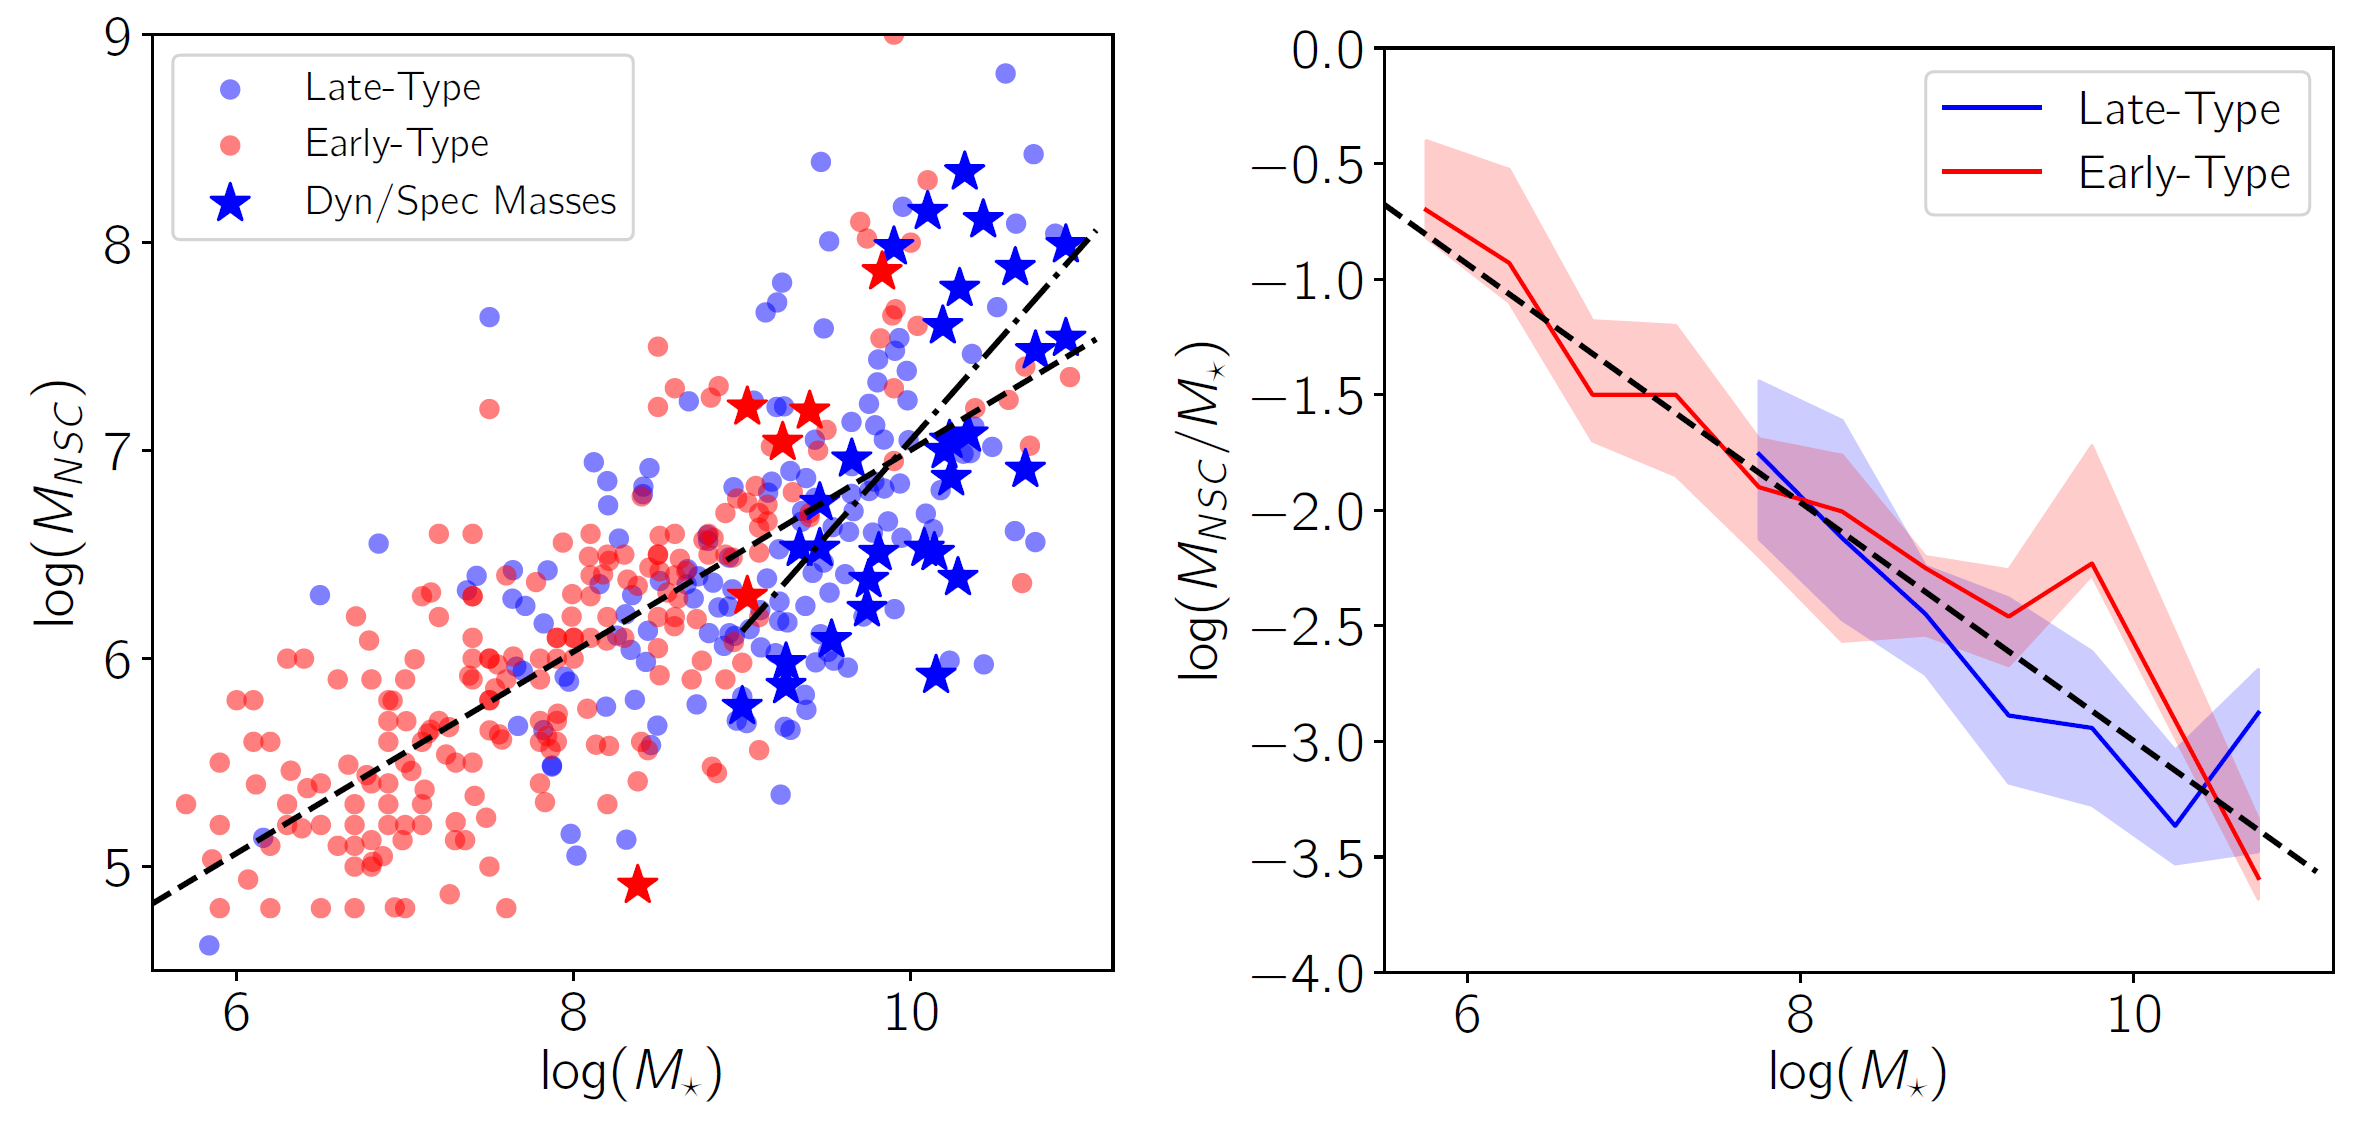
\includegraphics[width=1.0\textwidth]{images/nscrelation}
%    \caption{The masses of nuclear star clusters (NSCs) correlate with galaxy masses, but higher-mass galaxies have a lower fraction of their mass in their NSC. \emph{Left} -- NSC mass vs.\ Galaxy mass ($M_\star$). The disks and stars represent different methods of determining the masses of the NSCs, see the text for more information. The full sample is fitted to the dashed line, while the dashed-dotted line is a fit to the subset marked with blue stars. Galaxies have been divided by their Hubble types into early (red) and late (blue) types. \emph{Right}~-- The mass fraction of galaxies in NSCs as a function of galaxy mass, using the data from the left panel. The line indicates the median galaxy within each mass bin, while shaded regions show the 25th and 75th percentiles of the distribution. Adapted from \citet{neumayer:20} with permission.} % Fig. 12
%    \label{fig:nscrelation}
%\end{figure}
%
%In Figure~\ref{fig:nscrelation} in the left pane, the masses of the nuclear star clusters are shown in relation to the masses of their host galaxies. The disks and stars represent two different studies. The star symbols refer to a study done by \citet{erwin:12b} where the mass of the studied nuclear star clusters either have been dynamically measured or obtained by fitting multiple single stellar populations to high resolution spectra. The disks represent studies where multiple single stellar populations have been fitted to colours obtained through photometry \citep{georgiev:16,spengler:17,ordenesbriceno:18,sanchezjanssen:19}. %The concept of single stellar population will be described in more detail in the next section below on formation and evolution.
%
%Fitting the total sample to a linear relationship gives the dashed line seen in Figure~\ref{fig:nscrelation}, given by \citet{neumayer:20} as
%\begin{equation}
%    \log M_\textrm{NSC} = 0.48 \log \left( \frac{M_\textrm{host}}{10^9 \textrm{M}_\odot} \right) + 6.51.
%\end{equation}
%More simply put the mass of nuclear star clusters are proportional to the square root of the mass of their host galaxy. If one considers the methods used by \citet{erwin:12b} to be more accurate and precise then there more uncertain photometric based methods used by the other authors, and focus on late-type galaxies (i.e.\ spiral galaxies like the Milky Way) the relationship looks rather different, which is marked by the dashed-dotted line in Figure~\ref{fig:nscrelation}, given by \citet{neumayer:20} as
%\begin{equation}
%    \log M_\textrm{NSC} = 0.92 \log \left( \frac{M_\textrm{host}}{10^9 \textrm{M}_\odot} \right) + 6.13.
%\end{equation}
%Here the relation between the mass of the nuclear star clusters and their host galaxies is almost linear.
%
%Examining these relationships using the Milky Way data shows good agreement with either of the relations. They both adequately describe the relation between the mass of the Milky Way nuclear star cluster, $2.5 \cdot 10^7$\,M$_\odot$, and the mass of the Milky Way itself, $6 \cdot 10^{10}$\,M$_\odot$. In Figure~\ref{fig:nscrelation}, the Milky Way would be plotted near the intersection of the two lines.
%
%With an overview of galaxies in place, from a viewpoint that focuses on their centres, we turn our attention to their formation and evolution.
%
%\subsection{Formation and evolution of galaxies}
%
%Theories of formation and evolution of galaxies should be able to explain the galaxies we observe today, particularly the Milky Way, where observations provide much greater detail.
%
%With the advent of strong computational power in the last two decades, numerical simulations using first principles of fundamental physical laws combined with appropriate physical modelling have become one of the dominant methods for investigating galaxy formation and evolution \citep[see e.g.\ review by][]{naab:17}.
%
%The starting point for any theory of formation and evolution is the initial conditions. Modern cosmological models describe the Universe after the Big Bang and also how the structure of the Universe was initially formed. The initial baryonic matter in the Universe is described as a primordial gas consisting of hydrogen and helium, with helium having a mass fraction of about 24\% \citep{extragalacticbook}. The density of the primordial gas is not perfectly uniform initially, leading to the over-density regions amplifying with gravity over time to form the large scale structures, and finally the galaxies \citep[e.g.][]{mo:98}.
%
%In simulations based on cosmological models a Milky Way--like galaxy is typically formed by mergers of smaller galaxy fragments early on. Examples of such simulations are the EAGLE simulation \citep{eagle:i,eagle:ii}, the AURIGA simulation \citep{auriga:i} and the recent VINTERGATAN simulation \citep{vintergatan:i,vintergatan:ii,vintergatan:iii}.
%
%The limiting factor for simulations is computational power, and thus the different simulations vary in both the volume of space they cover and the shortest distances they can resolve in their simulated space. Furthermore, the simulations can be run multiple times to explore different initial conditions and increase statistics. The EAGLE simulation covers a very large volume of space, enough to contain about 10,000 Milky Way--mass galaxies, but has poor resolution ($\sim1$\,kpc). The AURIGA simulation focuses on simulating a single Milky Way--like galaxy, with intermediate resolution ($\sim200$\,pc), and runs the simulation 30 times with varying initial conditions to build up statistics. The VINTERGATAN simulation also focuses on simulating one Milky Way--like galaxy, having only one instance, but at very high resolution ($\sim20$\,pc).
%
%Alternatively, one can start with one large gas cloud and form a galaxy from that without accounting for the cosmological context, as a means of studying an isolated galaxy, which arguably the Milky Way could be. A recent example of such a simulation with multiple realisations has been done by \citet{khoperskov:20}, having a high resolution ($\sim50$\,pc).
%
%A major goal of the simulations mentioned above is to show how galaxies with a Milky Way--like morphology can be formed. While this is undoubtedly an important diagnostic, there are also other diagnostics available to us. One such diagnostic is the chemical composition of the atmospheres of the stars found in various parts of a galaxy. The underlying theories for this diagnostic are covered in more depth in Section~\ref{sect:chemicalevolution} on chemical evolution models. Common to the simulations mentioned above is that they all include this diagnostic, i.e.\ provide the chemical composition of the atmospheres of the stars found in the simulations.
%
%The chemical compositions of the atmospheres of stars can be observed in the Milky Way and its satellite dwarf galaxies where it is possible to resolve individual stars and determine their chemical composition using spectroscopy. It is not possible to resolve individual stars in other galaxies than these. However, with the advent of 30-40 meter telescopes now in construction, resolving stars in the neighbouring Andromeda galaxy, M31, should become possible \citep[see proposals by e.g.][]{escala:20}. This diagnostic is an example of how the greater detail of the Milky Way available to us enhances the demands on the theories.
%
%When discussing the chemical composition of the atmosphere of stars, one of the most commonly used approaches is to examine the ratio of alpha-abundance to iron-abundance of a star vs.\ the metallicity of the same star. The alpha-elements are the stable atoms with a nucleus comprised of a certain number of alpha-particles (2 neutrons and 2 protons), which are C, O, Ne, Mg, Si, S, Ar and Ca. The metallicity of stars is usually measured through the proxy of the ratio of iron to hydrogen abundance.
%
%In Figure~\ref{fig:vintergatan} and Figure~\ref{fig:khoperskovalpha} the alpha to iron-abundance vs.\ metallicity of respectively the VINTERGATAN simulation and one of the realisations from the \citet{khoperskov:20} simulations are shown. The really interesting and essential part is to compare these simulations with observations. These abundances have been observed in a stellar sample containing close to 300,000 stars in the APOGEE survey and an updated data version was released recently \citep{jonsson:20}. The abundance trends of the alpha-elements O, Mg and Si, with respect to Fe are shown in Figure~\ref{fig:dr16}.
%
%\begin{figure}[p]
%    \centering
%    \vspace{-0.5cm}
%    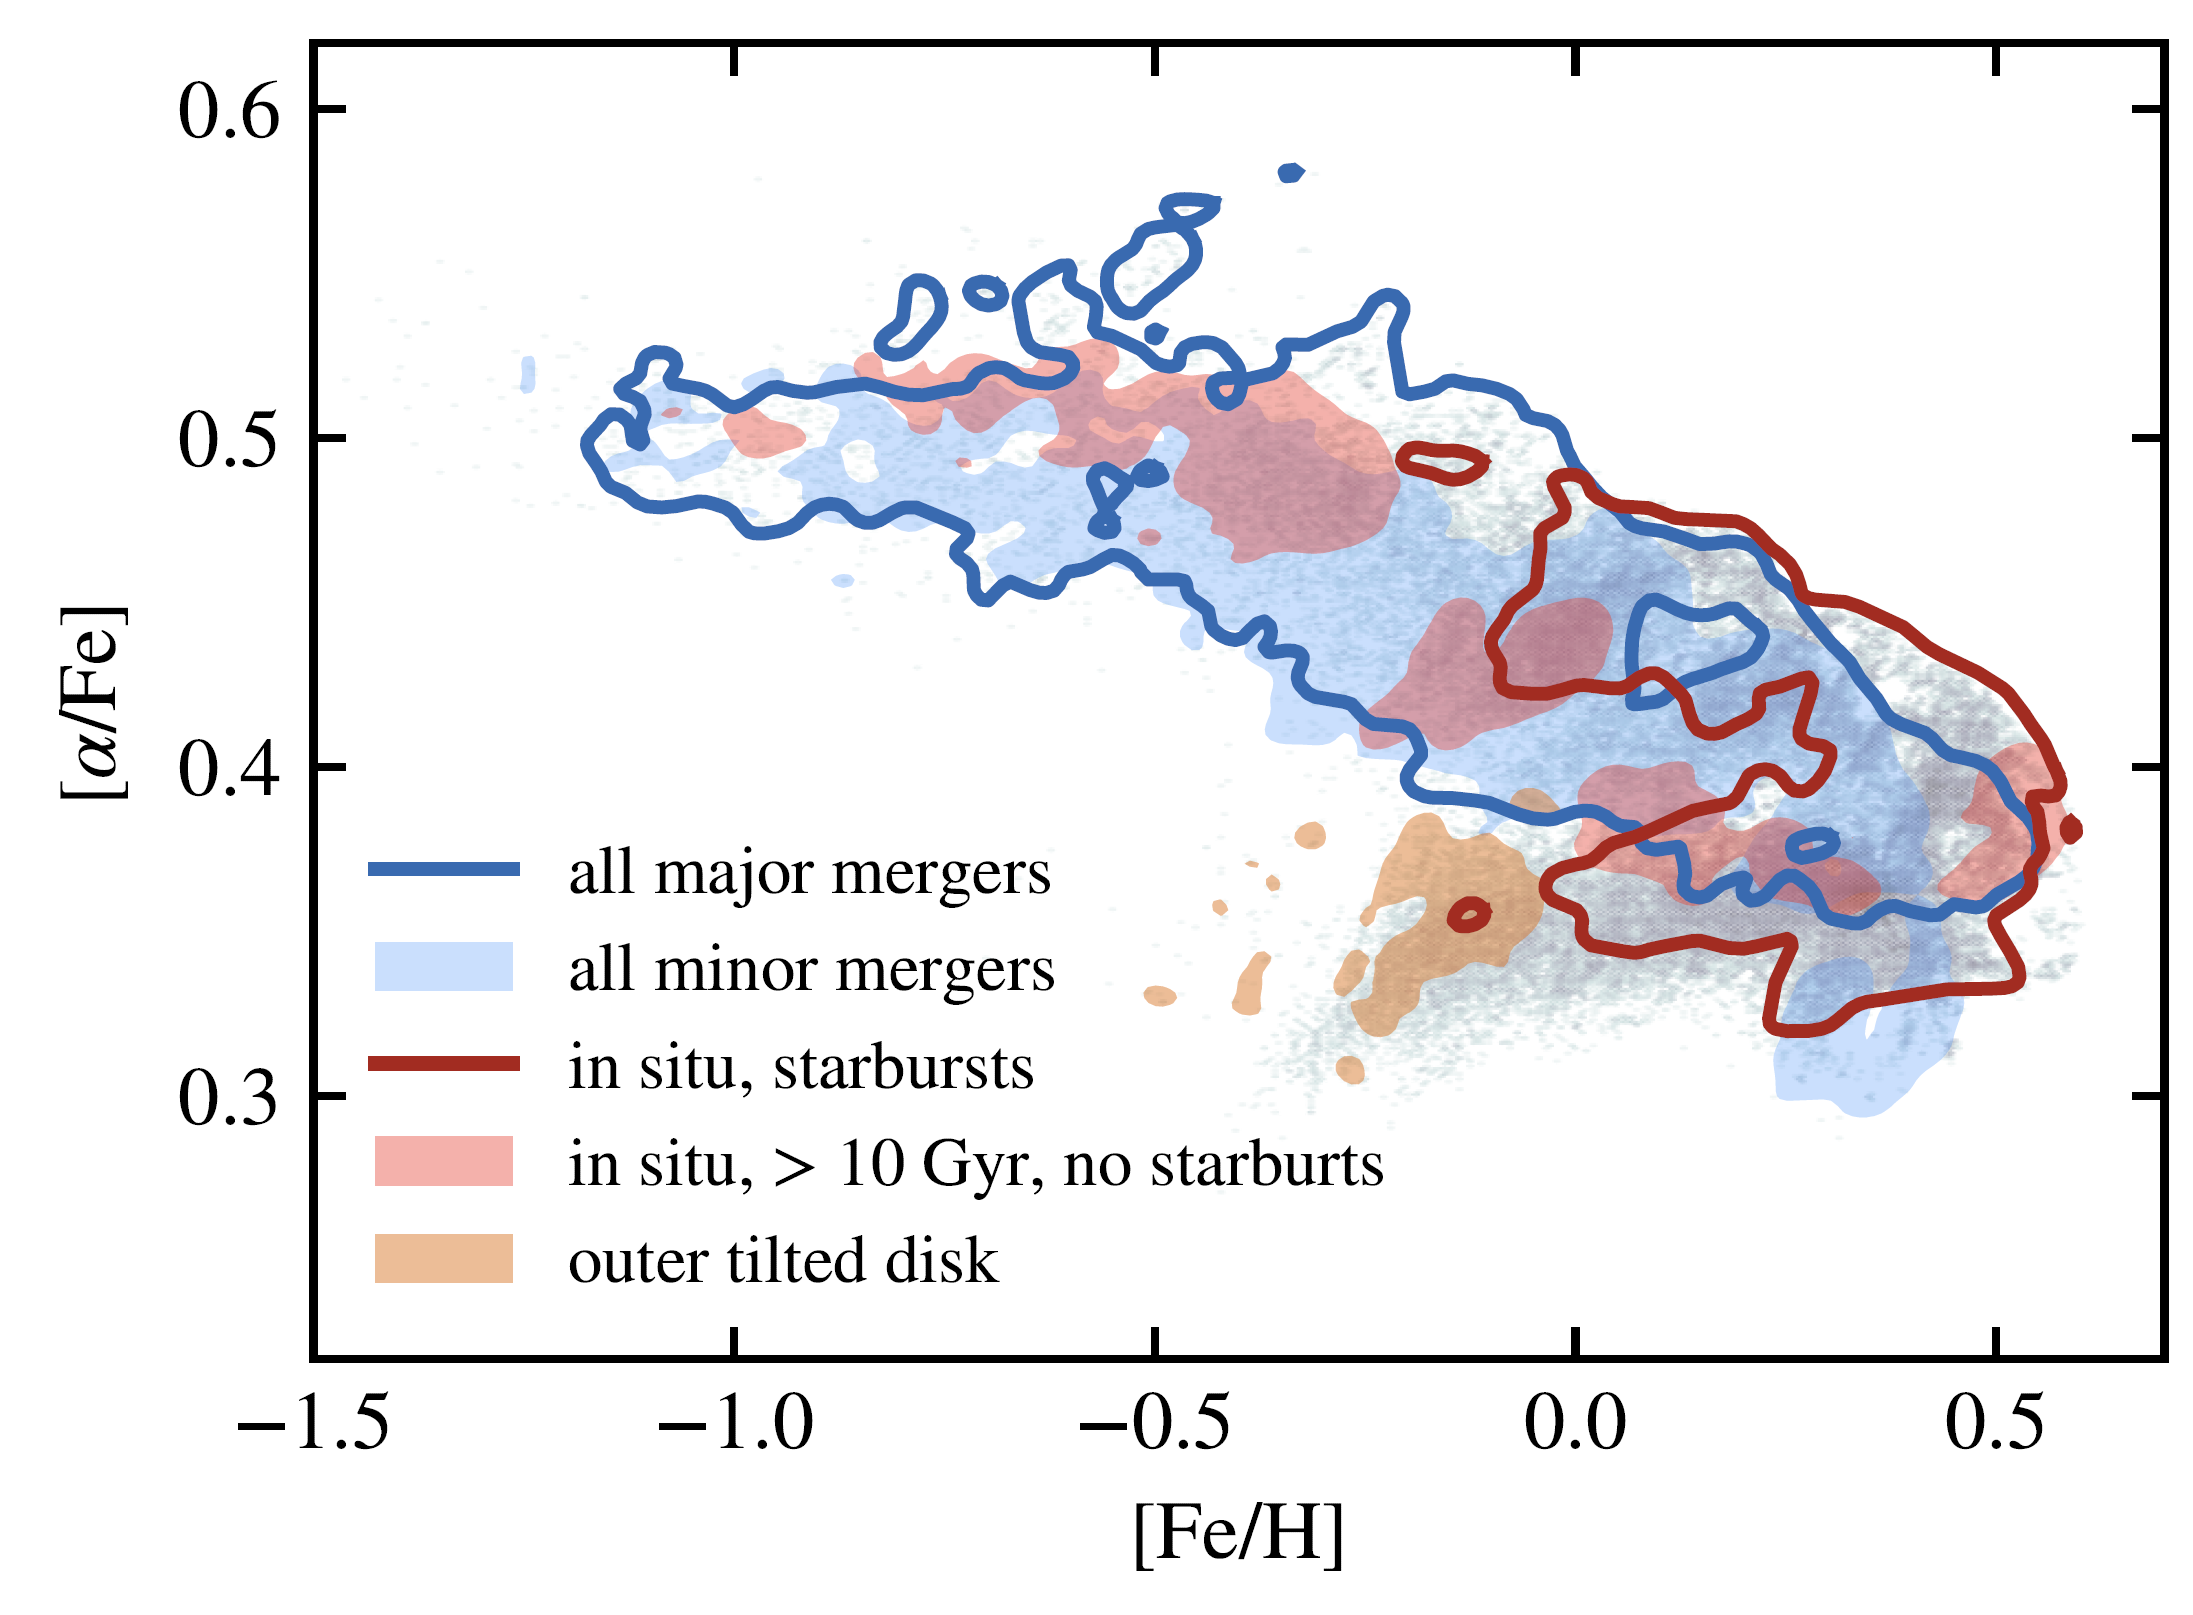
\includegraphics[width=0.8\textwidth]{images/vintergatan.png}
%    \vspace{-0.25cm}
%    \caption{Alpha-elements to iron abundances vs.\ metallicity, see text for explanation of notation. The grey dots in the background shows the chemical composition of stars found in the simulations with the coloured contours and regions mapping out the origin of their formation. Adapted from \citet{vintergatan:ii} with permission.} % Fig. 10
%    \label{fig:vintergatan}
%\end{figure}
%\begin{figure}[p]
%    \centering
%    \vspace{-0.5cm}
%    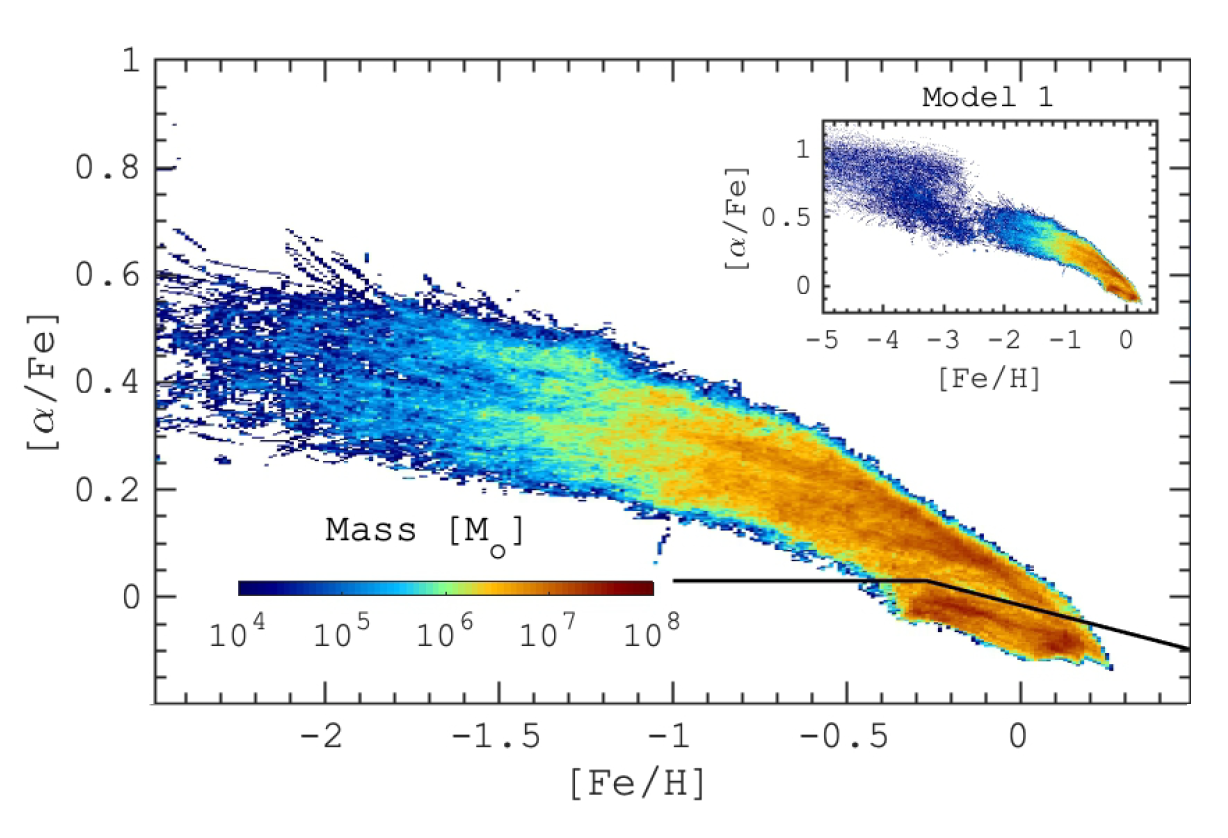
\includegraphics[width=0.8\textwidth]{images/khoperskovalpha.png}
%    \vspace{-0.25cm}
%    \caption{Alpha-elements to iron abundances vs.\ metallicity, colour-coded by the stellar mass, see text for explanation of notation. The frame in the top right is an overview of all the data in the simulation with the main figure itself a zoom-in. The black line separates two major stellar populations with low and high alpha-abundances. Adapted from \citet{khoperskov:20} with permission.} % Fig. 7
%    \label{fig:khoperskovalpha}
%\end{figure}
%\begin{figure}[p]
%    \centering
%    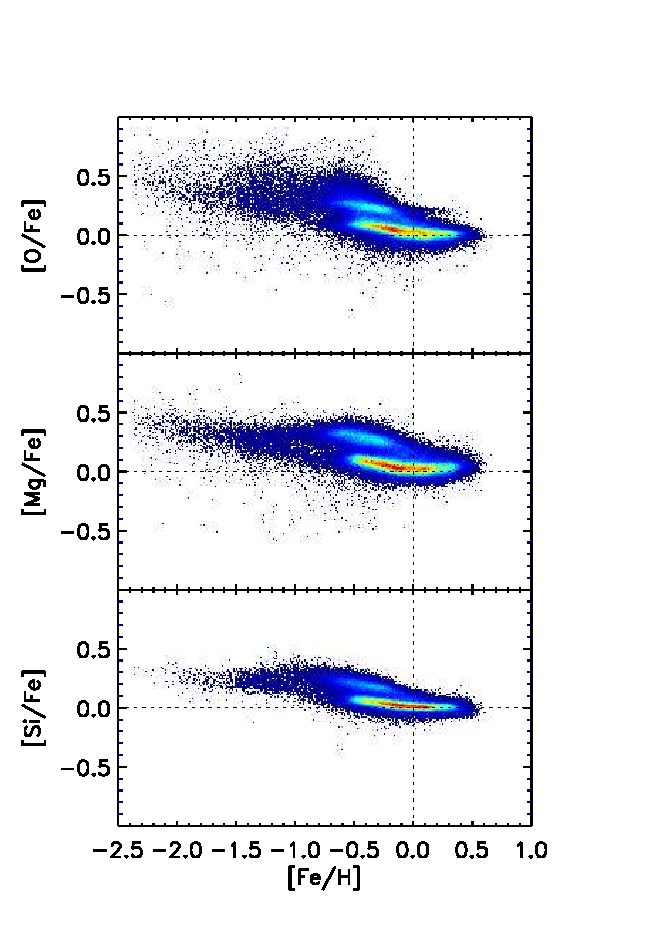
\includegraphics[trim={-0.3cm 0.9cm 0.8cm 1.8cm},clip,width=1.0\textwidth]{images/APOGEE_DR16_O_Mg_Si.pdf} % l b r t
%    \caption{Alpha-elements to iron abundances vs.\ metallicity, colour-coded by the stellar number density, see text for explanation of notation. The stars were observed as part of the APOGEE survey \citep{jonsson:20}, and shown here are the trends from giant stars for the three alpha-elements, O, Mg and Si. Figure from H.\ Jönsson (private communication).}
%    \label{fig:dr16}
%\end{figure}
%
%The notation [O/Fe] is to be understood as the abundance ratio of O to Fe logarithmically compared to the same ratio found in the Sun, as described by
%\begin{equation}
%    [\textrm{O}/\textrm{Fe}] = \log\left(\frac{N_\textrm{O}}{N_\textrm{Fe}}\right)_\textrm{star} - \log\left(\frac{N_\textrm{O}}{N_\textrm{Fe}}\right)_\textrm{Sun},
%\end{equation}
%where $N_\textrm{O}$ and $N_\textrm{Fe}$ are the number densities of O and Fe atoms respectively. The Sun is therefore located at the origin in the abundance plots. In Figure~\ref{fig:vintergatan} [\textalpha/Fe] is traced by [O/Fe] in the simulation, while in Figure~\ref{fig:khoperskovalpha} [\textalpha/Fe] is traced by the average of [O/Fe], [Mg/Fe] and [Si/Fe].
%
%Comparing the trends in Figures~\ref{fig:vintergatan} and \ref{fig:khoperskovalpha} to the trends in Figure~\ref{fig:dr16} shows the same high ratios that recede as the metallicity increases. In particular, the simulation can offer explanations for how the bimodal nature of the abundance trends arises from an evolution of the star formation activity in the galactic host. This is driven both by the transition from a merger-dominated growth phase in the early Universe to a quiescent evolution later, and the joint intrinsic evolution of the disks. Such matters are out of the scope of this thesis \citep[for details, see][]{vintergatan:ii}.
%
%\begin{figure}[t]
%    \centering
%    \vspace{-0.5cm}
%    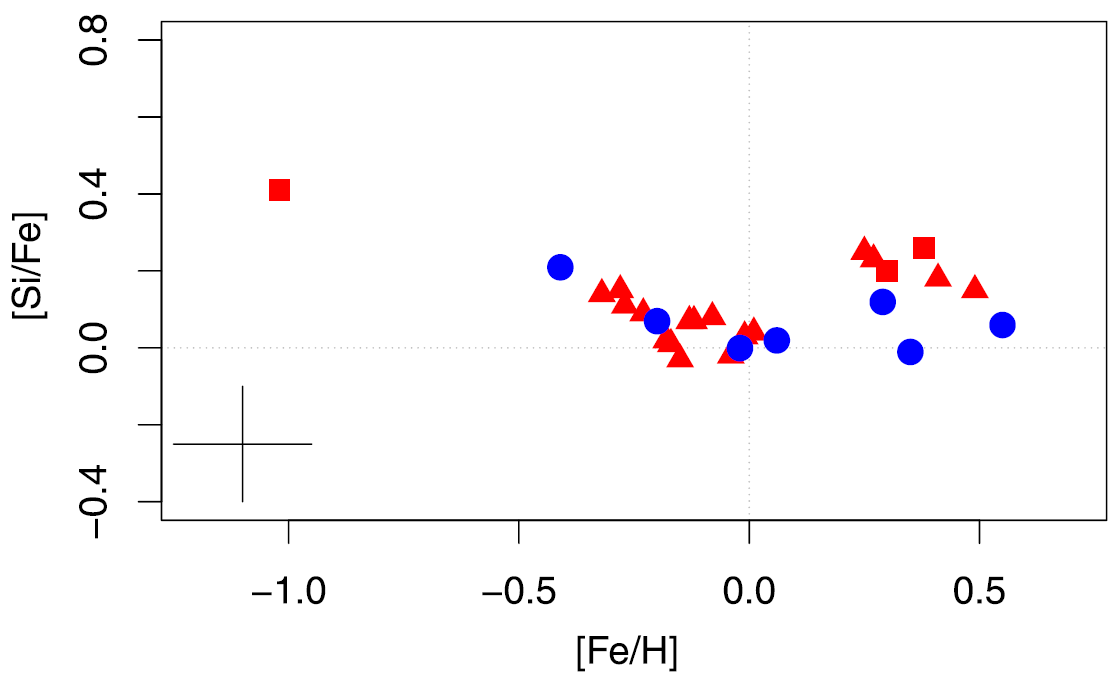
\includegraphics[width=0.8\textwidth]{images/thorsbroalpha.png}
%    \vspace{-0.25cm}
%    \caption{Alpha-elements to iron abundances vs.\ metallicity, here traced by Si, see text for explanation of notation. Red triangles and squares are abundances of stars found in the nuclear star cluster and nuclear stellar disk of the Milky Way; blue circles are stars found in the Milky Way disk. Adapted from \citet{thorsbro:20} with permission.} % Fig. 5
%    \label{fig:thorsbroalpha}
%\end{figure}
%
%The work in this thesis aims at adding observations of the Galactic centre to the available data. The data we have obtained is presented in the accompanying papers. One of our central results is shown here in Figure~\ref{fig:thorsbroalpha}. To our knowledge, there are currently no numerical simulations that have attempted to simulate the formation and evolution of the Galactic centre with a sufficient resolution to make a comparison to our data. In our Paper V we compare the data with chemical evolution models to offer possible interpretations of our data. It is our hope that with the availability of data like ours more theoretical work can be done to better understand the Galactic centre.

